\chapter{Introduction to \tls{}}

\label{sec:tlsintro}
\tls{} stands for 'Transport Layer Security' and is the successor of \ssl{},
the Secure Sockets Layer protocol\footnote{described in \cite{SSL3}} designed by Netscape. 
\tlsI{} is an Internet protocol,
defined by {IETF}\footnote{IETF or Internet Engineering Task Force 
is a large open international community of network
designers, operators, vendors, and researchers concerned with the evolution of 
the Internet architecture and the smooth operation of the Internet. It is open 
to any interested individual.}, described in \cite{RFC2246} and
also in \cite{RESCOLA}. The protocol provides confidentiality, and 
authentication layers over any reliable transport layer. The description, 
below, refers to \tlsI{} but also applies to \sslIII{} since the differences 
of these protocols are minor. Older protocols such as \sslII{} are not 
discussed nor implemented in \gnutls{} since they are not considered secure 
today.

\newpage
\section{TLS layers}

\tlsI{} is a layered protocol, and consists of the Record Protocol,
the Handshake Protocol and the Alert Protocol. The Record Protocol
is to serve all other protocols and is above the transport layer.
The Record protocol offers symmetric encryption, and data authenticity.
In \gnutls{} the record protocol is accessed using the 
\hyperref{gnutls\_record\_read()}{gnutls\_record\_read() (see Section }{)}{gnutls_record_read} and
\hyperref{gnutls\_record\_write()}{gnutls\_record\_write() (see Section }{)}{gnutls_record_write}
functions.

\par
The Alert protocol offers some signaling to the other protocols. It can
help informing the peer for the cause of failures and other error
conditions.
\hyperref{gnutls\_alert\_send()}{gnutls\_alert\_send() (see Section }{)}{gnutls_alert_send} and
\hyperref{gnutls\_alert\_send\_appropriate()}{gnutls\_alert\_send\_appropriate() (see Section }{)}{gnutls_alert_send_appropriate} 
functions.

\par 
The Handshake protocol is responsible for the initial key exchange,
and authentication. See \hyperref{figure}{figure }{}{fig:cert} for the
protocol layering in TLS. The handshake protocol in \gnutls{} is accessed
with the 
\hyperref{gnutls\_handshake()}{gnutls\_handshake() (see Section }{)}{gnutls_handshake} function.

\begin{figure}[hbtp]
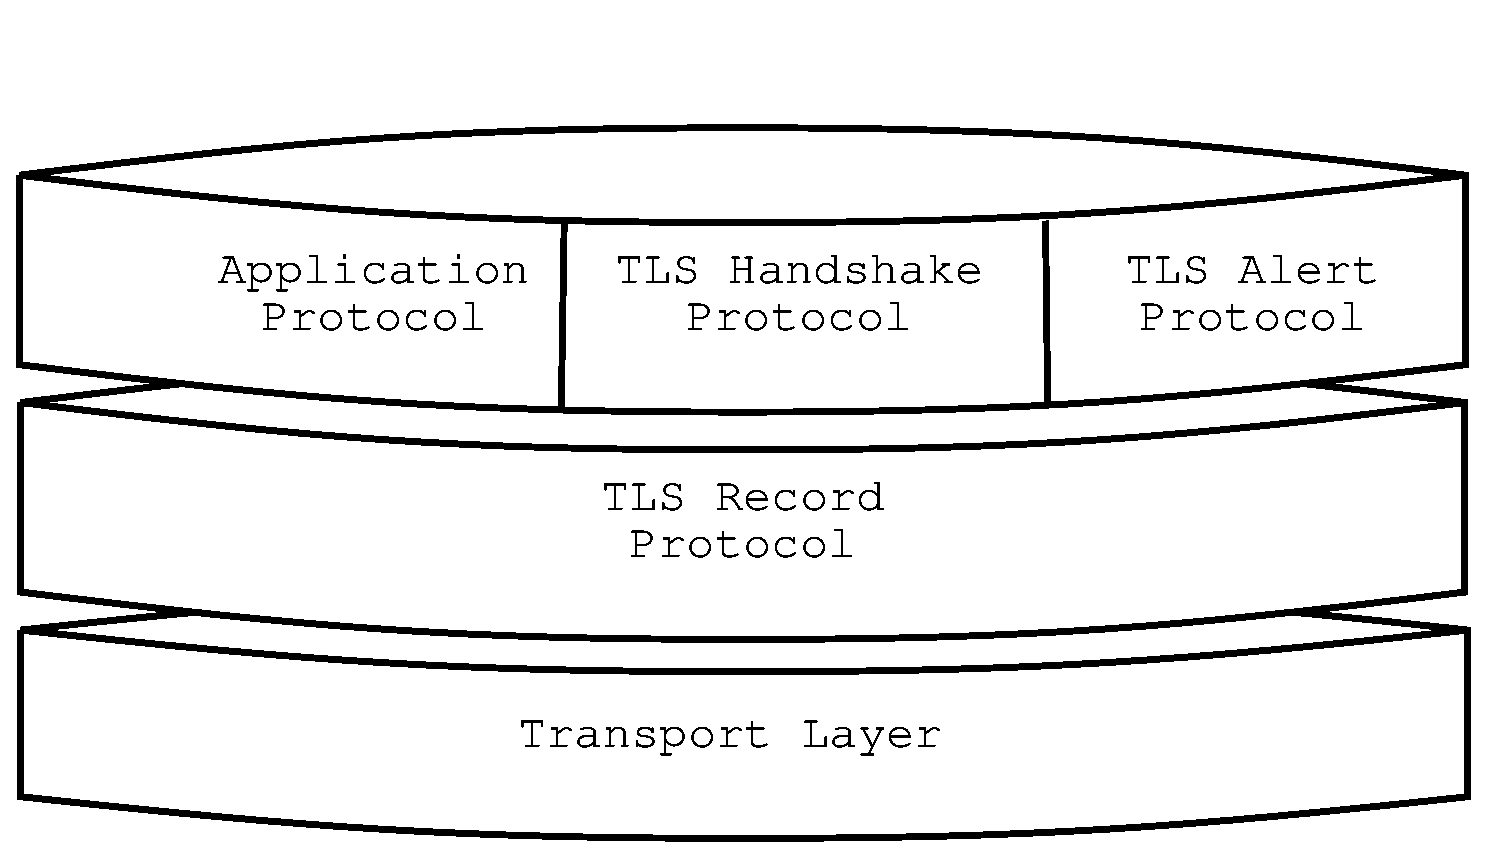
\includegraphics{layers}
\label{fig:layers}

\end{figure}


\addvspace{1.5cm}



\section{Transport Layer}
\par
\gnutls can be used above any transport layer. To do this you will only 
need to set up the 
\hyperref{gnutls\_transport\_set\_push\_function()}{gnutls\_transport\_set\_push\_function() (see Section }{
for more information)}{gnutls_transport_set_push_function} and
\hyperref{gnutls\_transport\_set\_pull\_function()}{gnutls\_transport\_set\_pull\_function() (see Section }{
for more information)}{gnutls_transport_set_pull_function}
functions. These functions will then be used by gnutls in order to send and receive data.
The functions specified should return -1 on error and should set errno appropriately.
\gnutls supports EINTR and EAGAIN errno values. These values are
usually used in non blocking IO and interrupted system calls.
The corresponding values (GNUTLS\_E\_INTERRUPTED, GNUTLS\_E\_AGAIN) 
will be returned to the caller of the gnutls function. \gnutls functions
can be resumed (called again), if any of these values is returned.
\par
By default (if none of the above functions are not called), gnutls will use
the berkeley sockets functions recv() and send(). In this case
gnutls will use some hacks in order for select() to work, thus
making easy to add {\emph TLS} support to existing servers.




\section{The TLS record protocol\index{TLS protocols!Record}}

The Record protocol is the secure communications provider. It's purpose
is to encrypt, authenticate and --optionally-- compress packets.
The following functions are available:
\par
\begin{itemize}
\item \printfunc{gnutls_record_send}{gnutls\_record\_send}:
to send a record packet (with application data).
\item \printfunc{gnutls_record_recv}{gnutls\_record\_recv}:
to receive a record packet (with application data).
\end{itemize}

As you may have already noticed, the functions which access the Record protocol,
are quite limited, given the importance of this protocol in \tls{}.
This is because the Record protocol's parameters are all set by
the Handshake protocol (see section \ref{handshake} on page \pageref{handshake}).
\par
The Record protocol initially starts with NULL parameters, which means
no encryption, and no MAC is used. Encryption and authentication begin
just after the handshake protocol has finished.

\subsection{Encryption algorithms used in the record layer}
\index{Symmetric encryption algorithms}
Confidentiality in the record layer is achieved by using symmetric block 
encryption algorithms like {\bf 3DES}, {\bf AES\footnote{AES or Advanced 
Encryption Standard is actually the RIJNDAEL algorithm. This is the
algorithm that replaced DES.}}, or
stream algorithms like {\bf ARCFOUR\_128\footnote{ARCFOUR\_128 is a compatible
algorithm with RSA's RC4 algorithm, which is considered to be a trade secret.}} See \hyperref{fig:ciphers}{figure }{}{fig:ciphers} for a complete list. 
Ciphers are encryption algorithms that use a single (secret) key
to encrypt and decrypt data. Block algorithms in TLS also provide protection
against statistical analysis of the data. \gnutls{} makes use of this property
thus, if you're using the \tlsI{} protocol, a random number of blocks will be
appended to the data. This will prevent eavesdroppers from guessing the 
actual data size.

\begin{figure}[hbtp]
\begin{tabular}{|l|p{9cm}|}

\hline
3DES\_CBC & 3DES\_CBC is the DES block cipher algorithm used with triple
encryption (EDE). Has 64 bits block size and is used in CBC mode.
\\
\hline
ARCFOUR\_128 & ARCFOUR is a fast stream cipher.
\\
\hline
ARCFOUR\_40 & This is the ARCFOUR cipher that is fed with a 40 bit key,
which is considered weak.
\\
\hline
AES\_CBC & AES or RIJNDAEL is the block cipher algorithm that replaces 
the old DES algorithm. Has
128 bits block size and is used in CBC mode. This is not officially
supported in TLS.
\\
\hline
\end{tabular}
\caption{Supported cipher algorithms}
\label{fig:ciphers}
\end{figure}



\addvspace{1.5cm}

\begin{figure}[hbtp]
\begin{tabular}{|l|p{9cm}|}

\hline
MAC\_MD5 & MD5 is a cryptographic hash algorithm designed by Ron Rivest. Outputs 128 bits of data.
\\
\hline
MAC\_SHA & SHA is a cryptographic hash algorithm designed by NSA. Outputs 160 bits of data.
\\
\hline
MAC\_RMD160 & RIPEMD is a cryptographic hash algorithm developed in the framework
of the EU project RIPE. Outputs 160 bits of data.
\\
\hline
\end{tabular}
\caption{Supported MAC algorithms}
\index{MAC algorithms}
\label{fig:mac}
\end{figure}



\subsection{Compression algorithms used in the record layer}
\index{Compression algorithms}
The TLS' record layer also supports compression. The algorithms
implemented in \gnutls{} can found in figure \ref{fig:compression}.
All the algorithms should be considered as \gnutls' extensions, and
should be advertised only when the peer is known to have a compliant client,
to avoid interoperability problems.
\par
The included algorithms perform really good when text, or other
compressable data are to be transfered, but offer nothing on already 
compressed data, such as compressed images, zipped archives etc.
These compression algorithms, may be useful in high bandwidth TLS tunnels,
and in cases where network usage has to be minimized. As a drawback, 
compression increases latency.

\begin{figure}[hbtp]
\begin{tabular}{|l|p{9cm}|}

\hline
ZLIB & ZLIB compression, using the deflate algorithm.
\\
\hline
LZO & LZO is a very fast compression algorithm. This algorithm is only
available if the \gnutlse{} library has been initialized.
\\
\hline
\end{tabular}
\caption{Supported compression algorithms}
\label{fig:compression}
\end{figure}




\subsection{Weaknesses and countermeasures}
\index{TLS protocols!Record}

Some weaknesses that may affect the security of the Record layer have been
found in \tlsI{} protocol. These weaknesses can be exploited by active attackers,
and exploit the facts that \tls{} 
\begin{enumerate}
\item has separate alerts for ``decryption\_failed'' and ``bad\_record\_mac''
\item the decryption failure reason can be detected by timing the responce time
\item the IV for CBC encrypted packets is the last block of the previous encrypted packet
\end{enumerate}

\gnutls{} implements all the known counter-measures for these attacks. For the first
two cases, \gnutls{} does only have one error code for both of the decryption failures,
and processes the message normaly even if a padding error occured. This avoids
both of these attacks.
For the latter, an empty record can be sent before every record packet, and this is
believed to avoid the known attacks in CBC encrypted packets. See the function
\printfunc{gnutls_record_set_cbc_protection}{gnutls\_record\_set\_cbc\_protection}
for more information.

For a detailed discussion see the archives of the TLS Working Group mailing list
and the paper \cite{CBCATT}.





\section{The TLS alert protocol}
\label{alert}

The Alert\index{TLS protocols!Alert} protocol
is there to allow signals to be sent between peers.
These signals are mostly used to inform the peer about the cause of
a protocol failure. Some of these signals are used internally by the
protocol and the application protocol does not have to cope with them
(see \emph{GNUTLS\_A\_CLOSE\_NOTIFY}), and others refer to the
application protocol solely (see \emph{GNUTLS\_A\_USER\_CANCELLED}).
An alert signal includes a level indication which may be either
fatal or warning. Fatal alerts always terminate the current connection,
and prevent future renegotiations using the current session ID.

\par The alert messages are protected by the record protocol, thus
the information that is included does not leak. You must take
extreme care for the alert information not to leak to a possible attacker
(via public log files etc).

\par
\begin{itemize}
\item \printfunc{gnutls_alert_send}{gnutls\_alert\_send}:
to send an alert signal.
\item \printfunc{gnutls_error_to_alert}{gnutls\_error\_to\_alert}:
to map a gnutls error number to an alert signal.
\item \printfunc{gnutls_alert_get}{gnutls\_alert\_get}:
returns the last received alert.
\item \printfunc{gnutls_alert_get_name}{gnutls\_alert\_get\_name}:
returns the name (in a character array) of the given alert.
\end{itemize}


\section{The handshake protocol}

The Handshake protocol is fully controlled by application layer (your 
program). Within this protocol the parameters for cipher suites, supported
authentication methods etc. are negotiated. Thus the application layer
has to set up the required parameters for the connection.
See the following functions:
\begin{itemize}
\item \printfunc{gnutls_cipher_set_priority}{gnutls\_cipher\_set\_priority()}:
to set the priority of bulk cipher algorithms.
\item \printfunc{gnutls_mac_set_priority}{gnutls\_mac\_set\_priority()}:
to set the priority of MAC algorithms.
\item \printfunc{gnutls_kx_set_priority}{gnutls\_kx\_set\_priority()}:
to set the priority of key exchange algorithms.
\item \printfunc{gnutls_compression_set_priority}{gnutls\_compression\_set\_priority()}:
to set the priority of compression methods.
\item \printfunc{gnutls_cert_type_set_priority}{gnutls\_cert\_type\_set\_priority()}:
to set the priority of certificate types (ie. OpenPGP, X.509).
\item \printfunc{gnutls_protocol_set_priority}{gnutls\_protocol\_set\_priority()}:
to set the priority of protocol versions (ie. \sslIII{}, \tlsI).
\item \printfunc{gnutls_cred_set}{gnutls\_cred\_set()}: to set the
appropriate credentials structures.
\item \printfunc{gnutls_certificate_server_set_request}
{gnutls\_certificate\_server\_set\_request()}: to set
whether client certificate is required or not.
\item \printfunc{gnutls_handshake}{gnutls\_handshake()}: to initiate the
handshake.
\end{itemize}

\subsection{Resuming Sessions}
\par
The 
\printfunc{gnutls_handshake}{gnutls\_handshake()}
 function, is expensive since a lot of calculations are performed. In order to support many fast connections to
the same server a client may use session resuming. {\bf Session resuming} is a
feature of the {\bf TLS} protocol which allows a client to connect to a server,
after a successful handshake, without the expensive calculations (by using the previously
established keys). \gnutls{} supports this feature, and the
example \hyperref{resume client}{resume client (see Section }{)}{resume-example} illustrates a typical use of it (This is a modification of the simple client example).
Servers only need to use the
\hyperref{gnutls\_db\_set\_name()}{gnutls\_db\_set\_name() (see Section }{)}{gnutls_db_set_name} function if they want to use the gdbm
backend to store sessions. 
\par
Keep in mind that sessions are expired after some time (for security reasons), thus
it may be normal for a server not to resume a session even if you requested that.
Also note that you must enable (using the priority functions), at least the
algorithms used in the last session.

\subsection{Resuming internals}
The resuming capability (mostly in the server side) is one of the problems of a thread-safe TLS
implementations. The problem is that all threads must share information in
order to be able to resume sessions. The gnutls approach is, in case of a
client, to leave all the burden of resuming to the client (ie. copy and keep the
nesessary parameters). See \hyperref{gnutls\_session\_get\_data()}
{gnutls\_session\_get\_data() on section }{}{gnutls_session_get_data},
\hyperref{gnutls\_session\_get\_id()}
{gnutls\_session\_get\_id() on section }{}{gnutls_session_get_id} and
\hyperref{gnutls\_session\_set\_data()}
{gnutls\_session\_set\_data() on section }{}{gnutls_session_set_data}.
\par
The server side is different.
Here the server only specifies a DB file, using 
\hyperref{gnutls\_db\_set\_name()}{gnutls\_db\_set\_name() (see Section }{)}{gnutls_db_set_name}.
This DB file is used to store the sessions' required parameters for
resuming. This means that this file contains very sensitive information,
such as encryption keys. In a multi-threaded application every thread can
read from the DB file and access all previously established sessions, but
only one thread can write at a time. The current behaviour of gnutls is
not to block to wait for the DB to be ready for writing, but continue the
process normally (and do not save the parameters).  
\par
 \gnutls{} also provides callback functions such as:
\hyperref{gnutls\_db\_set\_remove\_function()}{gnutls\_db\_set\_remove\_function() (see Section }{)}
{gnutls_db_set_remove_function}, 
\hyperref{gnutls\_db\_set\_store\_function()}{gnutls\_db\_set\_store\_function() (see Section }{)}
{gnutls_db_set_store_function}, \\
\hyperref{gnutls\_db\_set\_retrieve\_function()}{gnutls\_db\_set\_retrieve\_function() (see Section }{)
}{gnutls_db_set_retrieve_function} and 
\hyperref{gnutls\_db\_set\_ptr()}{gnutls\_db\_set\_ptr() (see Section }{)}
{gnutls_db_set_ptr}.
These callback functions are required in order to use a session
storage method, other than the default gdbm backend. 
\par
If an alternative backend is in use, it might be usefull to be able to check
for expired sessions in order to remove them, and save space. This is what
\hyperref{gnutls\_db\_clean()}{gnutls\_db\_clean() (see Section }{)}
{gnutls_db_clean} does for the gdbm backend. 
\gnutls{} provides the function
\hyperref{gnutls\_db\_check\_entry()}{gnutls\_db\_check\_entry() (see Section }{)
}{gnutls_db_check_entry}, which takes as input session data, and
returns a negative value if the data are to be removed.



\section{TLS Extensions}
\index{TLS Extensions}

A number of extensions to the \tls{} protocol have been proposed 
mainly in \cite{TLSEXT}. The extensions supported in \gnutls{} are
\begin{itemize}
\item Maximum fragment length negotiation
\item Server name indication
\end{itemize}
discussed in the subsections that follow.

\subsection*{Maximum fragment length negotiation}
\index{TLS Extensions!Maximum fragment length}

This extension allows a \tlsI{} implementation to negotiate
a smaller value for record packet maximum length. This extension
may be useful to clients with constrained capabilities. See
the 
\printfunc{gnutls_record_set_max_size}{gnutls\_record\_set\_max\_size}
and the 
\printfunc{gnutls_record_get_max_size}{gnutls\_record\_get\_max\_size}
functions.

\subsection*{Server name indication}
\index{TLS Extensions!Server name indication}

A common problem in HTTPS servers is the fact that the \tls{}
protocol is not aware of the hostname that a client connects to, when
the handshake procedure begins. For that reason the \tls{} server
has no way to know which certificate to send. This extension is hack
to the \tls{} protocol to allow the client to send the HTTP hostname
before the handshake begins --within the first handshake packet.

See the functions
\printfunc{gnutls_server_name_set}{gnutls\_server\_name\_set} and
\printfunc{gnutls_server_name_get}{gnutls\_server\_name\_get}.


